\documentclass{article}[14pt]
\usepackage[T2A]{fontenc}
\usepackage{geometry}
\usepackage{fancyhdr}
\usepackage{tocloft}
\usepackage{hyperref}
\usepackage{titlesec}
\usepackage{graphicx}
\usepackage{caption}
\usepackage{wrapfig}
\usepackage[english, russian]{babel}
\geometry{
	a4paper,
	top=20mm, 
	right=25mm, 
	bottom=25mm, 
	left=25mm
}
\usepackage{amssymb}
\usepackage{fancyvrb}
\usepackage{fvextra}
\usepackage{ dsfont }
\usepackage{amsmath}
\usepackage{listings}
\usepackage{xcolor}
\usepackage{listingsutf8}
\usepackage{pdfpages}
\usepackage{lipsum}
\usepackage{makecell}
\usepackage{float}
\usepackage{longtable}
\usepackage{tabularx}


\lstset{ 
	basicstyle=\ttfamily\small,
	keywordstyle=\color{blue},
	inputencoding=utf8,              
	extendedchars=true,
	stringstyle=\color{red}
	commentstyle=\color{green},
	showspaces=false,         
	showstringspaces=false,  
	numbers=left,              
	numberstyle=\tiny\color{gray},
	breaklines=true,          
	frame=single,           
	captionpos=b,             
	tabsize=4,
	escapeinside={(*@}{@*)}, % для работы с нестандартными текстами
	literate={ё}{{\"o}}1 {Ё}{{\"O}}1 {«}{{\guillemotleft}}1 {»}{{\guillemotright}}1
	{А}{{\CYRA}}1 {Б}{{\CYRB}}1 {В}{{\CYRV}}1 {Г}{{\CYRG}}1 {Д}{{\CYRD}}1 
	{Е}{{\CYRE}}1 {Ж}{{\CYRZH}}1 {З}{{\CYRZ}}1 {И}{{\CYRI}}1 {Й}{{\CYRISHRT}}1 
	{К}{{\CYRK}}1 {Л}{{\CYRL}}1 {М}{{\CYRM}}1 {Н}{{\CYRN}}1 {О}{{\CYRO}}1 
	{П}{{\CYRP}}1 {Р}{{\CYRR}}1 {С}{{\CYRS}}1 {Т}{{\CYRT}}1 {У}{{\CYRU}}1 
	{Ф}{{\CYRF}}1 {Х}{{\CYRH}}1 {Ц}{{\CYRC}}1 {Ч}{{\CYRCH}}1 {Ш}{{\CYRSH}}1 
	{Щ}{{\CYRSHCH}}1 {Ъ}{{\CYRHRDSN}}1 {Ы}{{\CYRERY}}1 {Ь}{{\CYRSFTSN}}1 
	{Э}{{\CYREREV}}1 {Ю}{{\CYRYU}}1 {Я}{{\CYRYA}}1 
	{а}{{\cyra}}1 {б}{{\cyrb}}1 {в}{{\cyrv}}1 {г}{{\cyrg}}1 {д}{{\cyrd}}1 
	{е}{{\cyre}}1 {ж}{{\cyrzh}}1 {з}{{\cyrz}}1 {и}{{\cyri}}1 {й}{{\cyrishrt}}1 
	{к}{{\cyrk}}1 {л}{{\cyrl}}1 {м}{{\cyrm}}1 {н}{{\cyrn}}1 {о}{{\cyro}}1 
	{п}{{\cyrp}}1 {р}{{\cyrr}}1 {с}{{\cyrs}}1 {т}{{\cyrt}}1 {у}{{\cyru}}1 
	{ф}{{\cyrf}}1 {х}{{\cyrh}}1 {ц}{{\cyrc}}1 {ч}{{\cyrch}}1 {ш}{{\cyrsh}}1 
	{щ}{{\cyrshch}}1 {ъ}{{\cyrhrdsn}}1 {ы}{{\cyrery}}1 {ь}{{\cyrsftsn}}1 
	{э}{{\cyrerev}}1 {ю}{{\cyryu}}1 {я}{{\cyrya}}1               
}
\begin{document}
	
\thispagestyle{empty}
\begin{center}
	\Large {\bfseries МИНИСТЕРСТВО НАУКИ И ВЫСШЕГО ОБРАЗОВАНИЯ РОССИЙСКОЙ ФЕДЕРАЦИИ}
	\\
	\vspace{3mm}
	Федеральное государственное автономное образовательное учреждение высшего образования <<Санкт-Петербургский политехнический университет Петра Великого>>
	\\
	\vspace{3mm}
	Институт компьютерных наук и кибербезопасности
	\\
	\vspace{3mm}
	Высшая школа технологий искусственного интеллекта
	\\
	\vspace{3mm}
	Направление: 02.03.01 Математика и компьютерные науки
	\\
	\vspace{2cm}
	\large{
		Методы тестирования программного обеспечения}
	\\
	\LARGE{
		Отчет по лабораторной работе №2\\
		<<Тестирование методом черного и белого ящика>>}
\end{center}

\vspace{5.5cm}
\begin{flushleft}
	\Large
	Студент
	\\
	группы 5130201/30101
	\\
	\vspace{2cm}
	\Large
	Преподаватель
	\\ 
\end{flushleft}
\vspace{-4.6cm}
\begin{flushright}
	\Large
	\line(1,0){2cm}
	\hspace{0.4cm}
	Шишмаков В.О.
	\\
	\vspace{2,7cm}
	\hspace{2cm}
	\Large
	\line(1,0){2cm}
	\hspace{0.4cm}
	Курочкин М. А.
	\hspace{-0.1cm}
	
\end{flushright}

\vspace{1cm}
\hspace{9.8cm}
{
	\Large
	\vspace{0.8cm}
	<<\underline{\hspace{1cm}}>>\underline{\hspace{2.5cm}} 2026 г.
}
\hfill \break
\hfill \break
\hfill \break
\hfill \break
\begin{center} \large{Санкт-Петербург, 2026} \end{center}
\pagebreak

\titleformat{\section}
{\Huge\bfseries}
{\thesection\;}
{0.65cm}
{}
\titleformat{\subsection}
{\huge\bfseries}
{\thesubsection\;}
{0.65cm}
{}
\titleformat{\subsubsection}
{\Large\bfseries}
{\thesubsubsection\;}
{0.65cm}
{}
\titlespacing*{\section}
{0em}
{1.5ex plus 1ex minus 0.2ex}
{1.5ex plus 1ex minus 0.2ex}	

\renewcommand*\contentsname{\huge{Содержание}}
\Large{
	\tableofcontents}
\pagebreak

\section*{Введение}
\addcontentsline{toc}{section}{Введение}

Одним из важнейших этапов в процессе создания современного программного обеспечения является тестирование. Выделяют 
различные виды тестирования: модульное, интеграционное, функциональное, системное и приемочное. В рамках данной работы 
основное внимание уделяется модульному тестированию.

Модульное тестирование представляет собой базовый вид проверки, с которого, как правило, начинается 
оценка корректности функционирования программы. Оно предполагает проверку отдельных компонентов программного продукта: 
классов, модулей и функций. Основная цель модульного тестирования — обнаружение дефектов, то есть случаев, когда реальное 
поведение модуля расходится с его спецификацией.

В практике модульного тестирования применяются два основных подхода: метод «черного ящика» и метод «белого ящика».

Оба этих подхода будут рассмотрены в данной работе.

\pagebreak

\section{Постановка задачи}

\noindent \textbf{Цель:} провести тестирование двух программ методами черного и белого ящика.

\noindent \textbf{Задачи:}

\begin{enumerate}
    \item Ознакомиться с подходами к модульному тестированию, а именно с методами черного и белого ящика.
    \item Составить тесты для двух программ и провести их.
    \item Провести анализ результатов тестирования.
\end{enumerate}

\pagebreak

\section{Описание методов тестирования}

\subsection{Метод черного ящика}

Одним из ключевых подходов к тестированию является метод «черного ящика», известный также как тестирование, 
ориентированное на данные, либо тестирование на основе входных и выходных параметров. Согласно данному подходу, 
программа рассматривается как <<черный ящик>>, внутренности и логика которого остаются скрыты и не 
принимаются во внимание. Основное внимание уделяется выявлению ситуаций, в которых реальная работа программы отклоняется 
от требований спецификации.

В рамках данного подхода необходимо выполнить проверку программы, используя такие техники, как разбиение входных данных на 
классы эквивалентности, анализ граничных значений и построение причинно-следственных диаграмм.

Далее будут подробно описаны три указанных приема тестирования методом «черного ящика».

\subsubsection{Эквивалентное разбиение}

Качественно разработанный тест должен охватывать значительную часть прочих потенциальных тестов, то есть предоставлять 
информацию о возможном присутствии или отсутствии дефектов в сценариях, не охваченных данным конкретным набором входных 
данных. В связи с этим целесообразно разделить все множество входных данных программы на ограниченное количество классов 
эквивалентности. Это позволит с достаточной уверенностью считать, что проверка на одном показательном значении из 
определенного класса равносильна проверке на любом другом значении из того же класса.

Процесс выделения классов эквивалентности заключается в последовательном анализе каждого входного условия 
и его разделении на две или более групп. Различают 
два типа классов эквивалентности: корректные классы, которые включают допустимые входные значения программы, и 
некорректные классы, представляющие все остальные возможные состояния.

Определение тестов по построенным классам эквивалентности состоит из трех этапов:

\begin{enumerate}
    \item Присвоить каждому классу эквивалентности номер.
    \item Разработать тесты, которые одновременно покрывают максимально возможное количество еще не задействованных 
    корректных классов, и продолжать этот процесс до тех пор, пока все корректные классы не будут охвачены.
    \item Создать тесты, каждый из которых покрывает ровно один из оставшихся некорректных классов, и повторять это 
    до полного охвата всех некорректных классов.
\end{enumerate}

\subsubsection{Анализ граничных значений}

Граничные условия представляют собой ситуации, которые возникают в окрестностях предельных значений, определяющих 
классы эквивалентности входных и выходных данных. Метод анализа граничных значений имеет два ключевых отличия от подхода, 
основанного на разбиении на классы эквивалентности.

\begin{enumerate}
    \item Вместо произвольного выбора любого значения из класса эквивалентности в качестве представителя всего класса, 
    анализ граничных значений требует выбора таких элементов, которые позволяют проверить именно каждую границу класса.
    \item При построении тестовых сценариев внимание уделяется не только входным данным (то есть области допустимых 
    входных значений), но и выходным данным (классам эквивалентности результатов).
\end{enumerate}

\subsubsection{Причинно-следственные диаграммы}

Причинно-следственная диаграмма представляет собой формализованный графический способ описания спецификации, 
изначально сформулированной на естественном языке. Базовая нотация таких диаграмм показана на рисунке 1. Каждый 
узел диаграммы может принимать одно из двух значений: 0 или 1, где 0 означает «отсутствует» или «ложно», а 1 --- 
«присутствует» или «истинно».

Данный метод призван восполнить недостаток подходов, основанных на анализе граничных значений и разбиении на классы 
эквивалентности, которые не учитывают комбинации входных условий.

Процесс построения тестов с использованием причинно-следственных диаграмм включает несколько шагов.

\begin{enumerate}
	\item Спецификация разделяется на фрагменты, более удобные для последующего анализа.
	\item В спецификации выделяются причины и следствия.

	\textbf{Причина} —-- это отдельное входное условие или класс эквивалентности входных данных.

	\textbf{Следствие} —-- это выходное условие либо изменение состояния системы (то есть долгосрочный эффект, который входное 
	воздействие оказывает на программу или систему).

	Выявление причин и следствий осуществляется путем тщательного изучения спецификации с подчеркиванием слов и фраз, 
	соответствующих этим понятиям. Каждой причине и каждому следствию присваивается уникальный идентификатор.

	\item Смысловое содержание спецификации анализируется и преобразуется в булев граф, отражающий связи между 
	причинами и следствиями. Полученный граф и есть причинно-следственная диаграмма.

	\item На диаграмму наносятся ограничения, которые описывают комбинации причин и/или следствий, невозможные в силу 
	синтаксических или внешних по отношению к программе условий.

	\begin{itemize}
		\item Ограничение E (исключающее) предусматривает, что из двух величин a и b только одна может принимать значение 1 
		(одновременное равенство единице запрещено, однако допустима ситуация, когда оба равны 0).
		\item Ограничение I (включающее) требует, чтобы хотя бы одна из величин a, b или c имела значение 1 
		(то есть запрещён случай, когда все три одновременно равны 0).
		\item Ограничение O (ровно одно) означает, что ровно одна из двух величин a или b должна быть равна 1.
		\item Ограничение R (требует) устанавливает, что a может быть равно 1 только в том случае, если b также равно 1 
		(иначе говоря, при b = 0 значение a не может быть 1). На рисунке 2 приведены условные обозначения для этих ограничений.
	\end{itemize}

	\item Посредством последовательного анализа состояний условий диаграмма преобразуется в ограниченную таблицу решений. 
	Каждый столбец этой таблицы соответствует отдельному тестовому сценарию.

	\item Столбцы полученной таблицы решений служат основой для формирования конкретных тестов.
\end{enumerate}

Базовая нотация причинно-следственных диаграмм представлена на рисунке \ref{fig:notation}.

\begin{figure}[H]
	\centering
	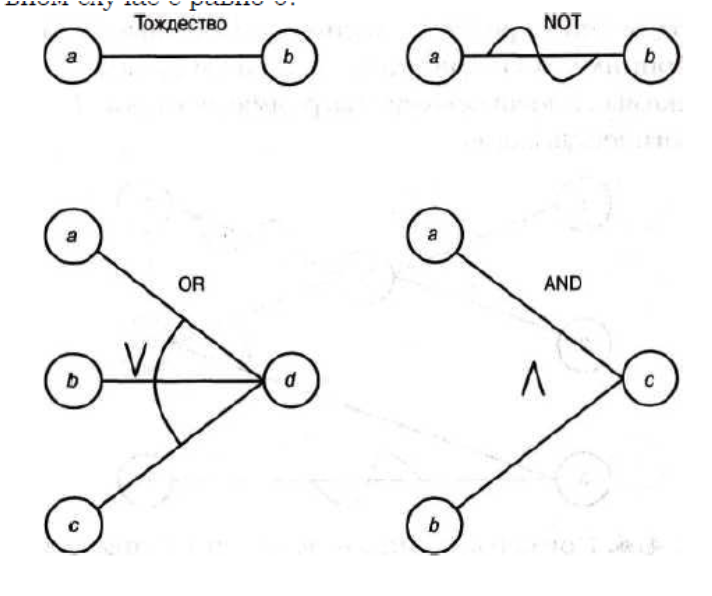
\includegraphics[width=0.6\textwidth]{pics/notaion.png}
	\captionof{figure}{Базовая нотация для причинно-следственных диаграмм}
	\label{fig:notation}
\end{figure}

Процедура заполнения очередного столбца таблицы решений выполняется следующим образом.

\begin{enumerate}
	\item Выбрать следствие, которое должно находиться в состоянии 1.
	\item Двигаясь по связям диаграммы от выбранного узла в обратном направлении, определить комбинации причин 
	(с учетом наложенных ограничений), которые приводят к установке этого следствия в 1.

	\begin{itemize}
		\item Если при обратном проходе встречается элемент OR, на выходе которого требуется получить 1, то 
		не следует одновременно устанавливать в 1 более одного входа этого элемента.
		\item Если при обратном проходе встречается элемент AND, на выходе которого требуется получить 0, то 
		необходимо перечислить все возможные комбинации входов, дающие на выходе 0. Однако при анализе ситуации, 
		где один из входов равен 0, а один или несколько других входов равны 1, нет необходимости перечислять 
		все варианты состояний остальных входов, равных 1.
		\item Если при обратном проходе встречается элемент AND, на выходе которого требуется получить 0, то достаточно 
		указать только одно условие, при котором все входы являются нулями.
	\end{itemize}

	\begin{figure}[H]
		\centering
		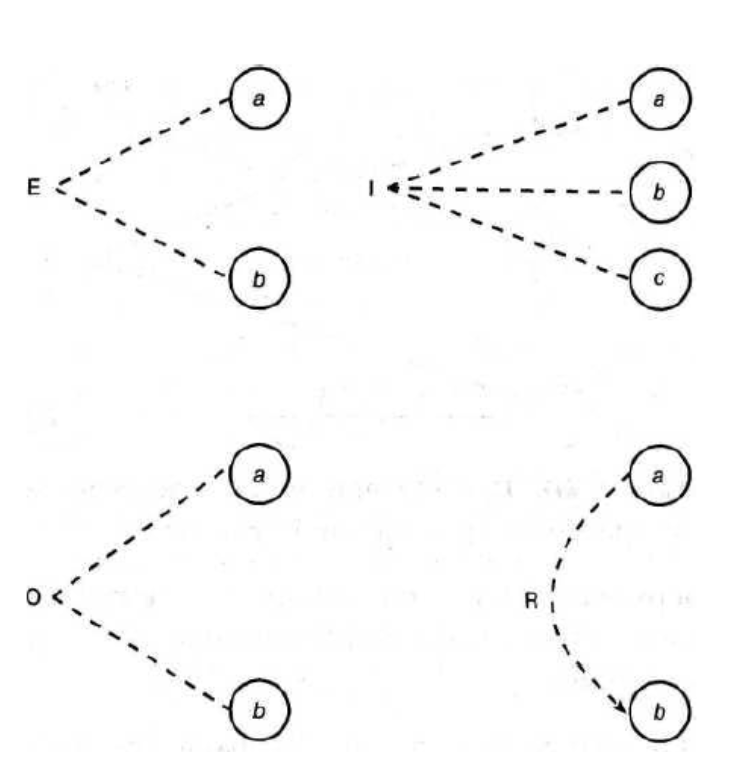
\includegraphics[width=0.6\textwidth]{pics/notation2.png}
		\captionof{figure}{Базовая нотация ограничений для причинно-следственных
диаграмм}
	\end{figure}

	\item Для каждой выявленной комбинации причин формируется отдельный столбец в таблице решений.
	\item Для каждой такой комбинации определяются состояния всех остальных следствий, которые затем заносятся в 
	соответствующий столбец таблицы.
\end{enumerate}

\subsection{Метод белого ящика}

В рамках подхода, известного как тестирование методом <<белого ящика>>, предоставляется возможность изучать внутреннее 
устройство программы. Основываясь на этом принципе, специалист по тестированию выбирает входные данные, анализируя 
логическую структуру программы.

Необходимо выполнить проверку программы, используя описанные ниже методы.

\subsubsection{Покрытие операторов}

Минимальным требованием к тестированию методом «белого ящика» является выполнение каждого оператора программы как минимум 
однократно. Однако, хотя это условие и необходимо, его недостаточно для обеспечения полноценной проверки.

\subsubsection{Покрытие решений}

Согласно данному критерию, необходимо подобрать такой набор тестов, при котором каждое логическое условие в программе 
хотя бы один раз принимает значение <<истина>> и хотя бы один раз —-- <<ложь>>. Другими словами, каждая возможная ветвь 
для всех инструкций, реализующих ветвление, должна быть пройдена минимум однократно.

\subsubsection{Покрытие условий}

Этот критерий требует, чтобы набор тестов обеспечивал для каждого элементарного условия, входящего в состав составного 
условия в точке ветвления, выполнение как минимум один раз значения <<истина>> и один раз значения <<ложь>>.

\subsubsection{Покрытие решений и условий}

В соответствии с данным критерием тестовый набор считается достаточным, если выполнены следующие условия: каждое 
элементарное условие внутри составного решения принимает оба возможных логических значения хотя бы однажды; каждый 
возможный результат самого решения также достигается минимум один раз; и каждая точка входа в программу или 
модуль активируется по крайней мере однократно.

\subsubsection{Комбинаторное покрытие условий}

Данный критерий предполагает формирование такого набора тестов, который обеспечивает проверку всех возможных комбинаций 
значений элементарных условий в каждом логическом решении, а также активацию каждой точки входа в программу как минимум 
однократно.

\pagebreak

\section{Тестирование программы №1}

\subsection{Описание программы}

\noindent \textbf{Автор:} Митяев Олег.

\noindent \textbf{Название:} Проверка простоты числа.

\noindent \textbf{Входные данные:}
\begin{itemize}
    \item $n$ --- строка, введённая пользователем; интерпретируется как целое число.
\end{itemize}

\noindent \textbf{Требуется:} определить, является ли число $n$ простым, и вывести соответствующее сообщение.

\noindent \textbf{Ограничения:}
\begin{enumerate}
    \item Введённая строка преобразуется в тип \texttt{int}. Если преобразование невозможно, выводится \texttt{ошибка ввода} и программа завершается.
    \item Числа $n \leq 1$ считаются непростыми.
    \item Число $n = 2$ является простым (частный случай).
    \item Чётные числа $n > 2$ считаются непростыми.
    \item Проверка простоты выполняется перебором нечётных делителей, начиная с $d = 3$ с шагом $2$, до $\lfloor\sqrt{n}\rfloor$ включительно.
\end{enumerate}

\noindent \textbf{Спецификация:}

\begin{table}[H]
\centering
\begin{tabular}{|p{2.5cm}|p{3.5cm}|p{2.5cm}|p{4cm}|}
\hline
\textbf{Входные данные} & \textbf{Ожидаемый результат} & \textbf{Статус} & \textbf{Комментарий} \\
\hline
7 & вывод: простое & Корректно & Обычный случай (простое число). \\
\hline
4 & вывод: не простое & Корректно & Обычный случай (составное число). \\
\hline
2 & вывод: простое & Корректно & Граница: минимальное простое. \\
\hline
1 & вывод: не простое & Корректно & Граница: $n \leq 1$ непростое. \\
\hline
-5 & вывод: не простое & Корректно & Отрицательные числа непростые. \\
\hline
abc & вывод: ошибка ввода; ожидание повторного ввода & Ошибка ввода & Проверка обработки некорректного ввода (строка вместо числа). \\
\hline
80 12 & вывод: ошибка ввода; ожидание повторного ввода & Ошибка ввода & Обработка некорректного ввода (число разделено пробелом). \\
\hline
3.45 & вывод: ошибка ввода; ожидание повторного ввода & Ошибка ввода & Обработка некорректного ввода (не целое число). \\
\hline
\end{tabular}
\end{table}

\begin{figure}[H]
	\centering
	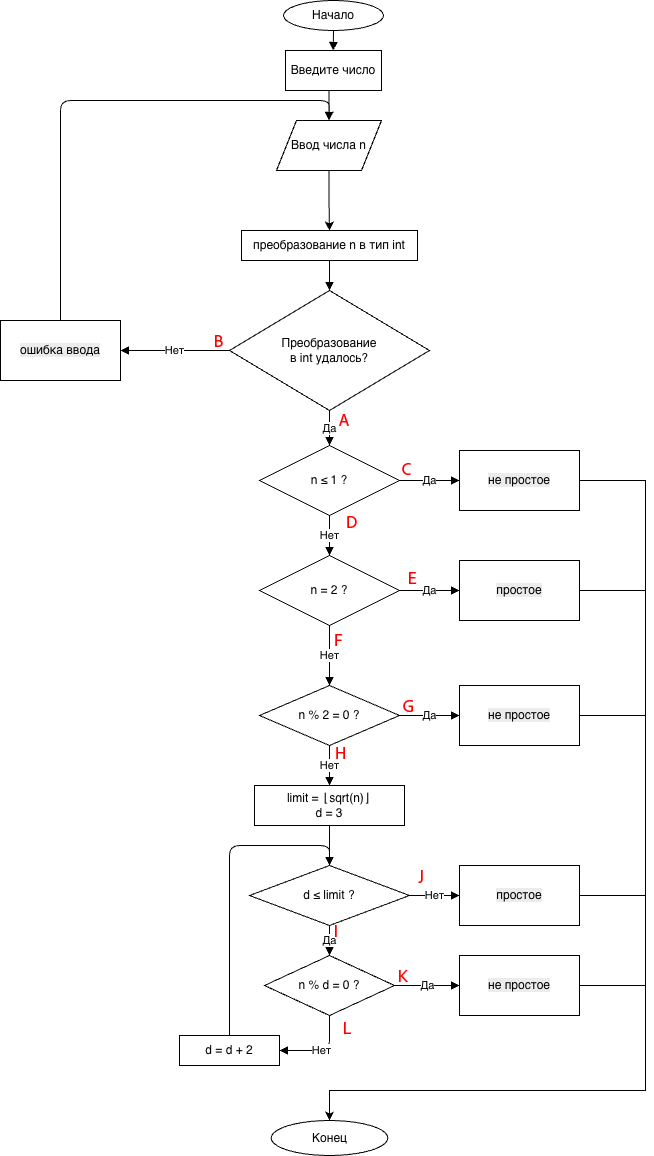
\includegraphics[width=0.8\textwidth]{pics/scheme1.png}
	\captionof{figure}{Блок-схема}
\end{figure}

\subsection{Тестирование методом <<черного>> ящика}

\subsubsection{Разбиение на классы эквивалентности}

Составлено разбиение на классы эквивалентности, исходя из ограничений для тестируемой программы.

{\centering\large{
\begin{longtable}{|p{4.5cm}|p{5.5cm}|p{5.5cm}|}
	\caption{Классы эквивалентности для n}\\
	\hline
	Входное условие & Допустимые классы & Недопустимые классы \\ \hline
	Целое число $n$ & Отрицательное число (1) & Нецелое вещественное число (8) \\ \hline
	& Ноль (2) & Строка (буквы) (9) \\ \hline
	& Единица (3) & Несколько чисел через пробел (10) \\ \hline
	& Минимальное простое (4) & Пустая строка (11) \\ \hline
	& Четное число $>2$ (5) & Спецсимволы / смешанный ввод (12) \\ \hline
	& Нечетное простое число (6) & \\ \hline
	& Нечетное составное число (7) & \\ \hline
\end{longtable}}}

В таблице \ref{tab:test-black-box-equivalents} представлены тесты, покрывающие все классы эквивалентности.

{\centering\large{
\begin{longtable}{|p{0.4cm}|p{0.8cm}|p{3cm}|p{3.5cm}|p{3.5cm}|p{2cm}|}
	\caption{Тесты, покрывающие классы эквивалентности}
	\label{tab:test-black-box-equivalents}\\
	\hline
	N & n & Класс эквивалентности & Ожидаемый результат & Фактический результат & Результат \\ \hline
	1 & -5 & (1) & Число не простое & Число не простое & Пройден \\ \hline
	2 & 0 & (2) & Число не простое & Число не простое & Пройден \\ \hline
	3 & 1 & (3) & Число не простое & Число не простое & Пройден \\ \hline
	4 & 2 & (4) & Число простое & Число простое & Пройден \\ \hline
	5 & 8 & (5) & Число не простое & Число не простое & Пройден \\ \hline
	6 & 17 & (6) & Число простое & Число простое & Пройден \\ \hline
	7 & 15 & (7) & Число не простое & Число не простое & Пройден \\ \hline
	8 & 7.5 & (8) & Ошибка ввода; повторный ввод & Ошибка ввода; повторный ввод & Пройден \\ \hline
	9 & abc & (9) & Ошибка ввода; повторный ввод & Ошибка ввода; повторный ввод & Пройден \\ \hline
	10 & 12 5 & (10) & Ошибка ввода; повторный ввод & Ошибка ввода; повторный ввод & Пройден \\ \hline
	11 & <<>> & (11) & Ошибка ввода; повторный ввод & Ошибка ввода; повторный ввод & Пройден \\ \hline
	12 & 10a? & (12) & Ошибка ввода; повторный ввод & Ошибка ввода; повторный ввод & Пройден \\ \hline
\end{longtable}}}

Все 12 тестов прошли успешно.

\subsubsection{Анализ граничных условий}

Исходя из ограничений данной программы можно выделить следующие граничные значения с точки зрения алгоритма:

\begin{enumerate}
    \item Переход от наибольшего непростого к наименьшему простому ($0$, $1$, $2$).
    \item Переход между наименьшим чётным составным и наименьшим нечётным простым ($2$, $3$, $4$).
    \item Делитель ровно на границе $\sqrt{n}$: $\sqrt{9} = 3$ ($8$, $9$, $10$).
    \item Граница корректности ввода: пустая строка, нечисловое значение, вещественное число.
\end{enumerate}

Для каждой из границ составлены тесты, соответствующие граничащим значениям.

\begin{table}[H]
\centering
\caption{Проверка граничных условий}
\begin{tabular}{|c|c|p{3.5cm}|p{3.5cm}|c|}
\hline
\textbf{N} & \textbf{n} & \textbf{Ожидаемый результат} & \textbf{Фактический результат} & \textbf{Результат} \\
\hline
1 & \texttt{0}   & Число не простое & Число не простое & Пройден \\
\hline
2 & \texttt{1}   & Число не простое & Число не простое & Пройден \\
\hline
3 & \texttt{2}   & Число простое    & Число простое    & Пройден \\
\hline
4 & \texttt{3}   & Число простое    & Число простое    & Пройден \\
\hline
5 & \texttt{4}   & Число не простое & Число не простое & Пройден \\
\hline
6 & \texttt{8}   & Число не простое & Число не простое & Пройден \\
\hline
7 & \texttt{9}   & Число не простое & Число не простое & Пройден \\
\hline
8 & \texttt{10}  & Число не простое & Число не простое & Пройден \\
\hline
9 & \texttt{\ }  & ошибка ввода     & ошибка ввода     & Пройден \\
\hline
10 & \texttt{abc} & ошибка ввода    & ошибка ввода     & Пройден \\
\hline
11 & \texttt{3.14} & ошибка ввода   & ошибка ввода     & Пройден \\
\hline
\end{tabular}
\end{table}

При проведении тестирования программа успешно обработала все граничные условия.

\subsubsection{Причинно-следственная диаграмма}

Для построения причинно-следственной диаграммы введём следующие обозначения:

\textbf{Причины:}
\begin{enumerate}
    \item Ввод является целым числом.
    \item Число $n \leq 1$.
    \item Число $n = 2$.
    \item Число $n$ чётное и $n \neq 2$.
    \item Среди нечётных чисел от $3$ до $\lfloor\sqrt{n}\rfloor$ найден делитель $n$.
\end{enumerate}

\textbf{Следствия:}
\begin{enumerate}
    \setcounter{enumi}{20}
    \item Программа выводит сообщение об ошибке ввода и запрашивает повторный ввод.
    \item Программа выводит результат: \texttt{не простое} (по условию $n \leq 1$).
    \item Программа выводит результат: \texttt{простое} (граничный случай $n = 2$).
    \item Программа выводит результат: \texttt{не простое} (чётное число $n \neq 2$).
    \item Программа выводит результат: \texttt{не простое} (найден делитель при переборе).
    \item Программа выводит результат: \texttt{простое} (делитель не найден).
\end{enumerate}

\textbf{Промежуточные узлы:}
\begin{enumerate}
    \setcounter{enumi}{10}
    \item Причина 1 истинна И причина 2 ложна
          (корректный ввод, $n > 1$ — число допущено к дальнейшему анализу).
    \item Узел 11 истинен И причина 3 ложна И причина 4 ложна
          (число нечётное и больше $2$ — выполняется перебор делителей).
\end{enumerate}

\textbf{Логические связи:}
\begin{enumerate}
    \item Следствие 21 (ошибка ввода) истинно, если причина 1 ложна
          (введено не целое число).
    \item Следствие 22 (\texttt{не простое}) истинно, если узел 11 ложен
          И причина 2 истинна (корректный ввод, $n \leq 1$).
    \item Следствие 23 (\texttt{простое}) истинно, если узел 11 истинен
          И причина 3 истинна ($n = 2$).
    \item Следствие 24 (\texttt{не простое}) истинно, если узел 11 истинен
          И причина 4 истинна (чётное $n \neq 2$).
    \item Следствие 25 (\texttt{не простое}) истинно, если узел 12 истинен
          И причина 5 истинна (при переборе найден делитель).
    \item Следствие 26 (\texttt{простое}) истинно, если узел 12 истинен
          И причина 5 ложна (делитель при переборе не найден).
    \item Узел 11 является конъюнкцией (AND) причин 1 и $\neg$2.
    \item Узел 12 является конъюнкцией (AND) узла 11, $\neg$3 и $\neg$4.
\end{enumerate}

\begin{figure}[H]
	\centering
	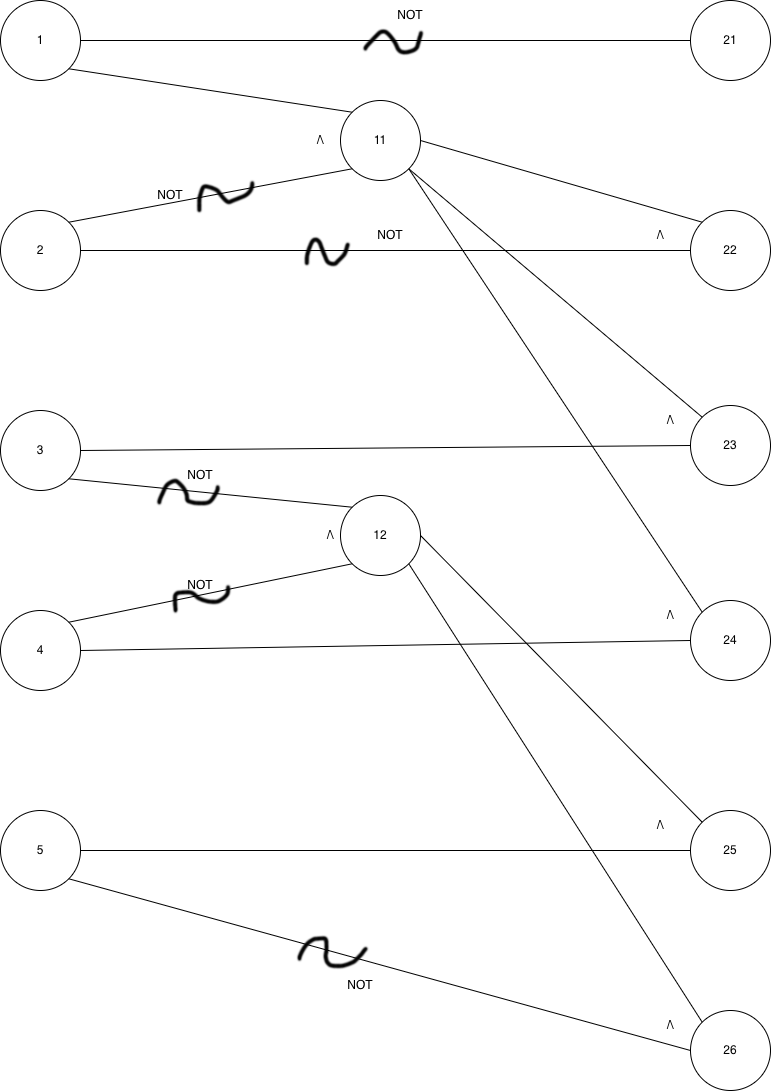
\includegraphics[width=0.6\textwidth]{../diagram2.png}
	\captionof{figure}{Причинно-следственная диаграмма}
\end{figure}

\begin{table}[H]
\centering
\caption{Таблица решений}
\renewcommand{\arraystretch}{1.4}
\begin{tabular}{|l|c|c|c|c|c|c|c|}
\hline
 & \textbf{1} & \textbf{2} & \textbf{3} & \textbf{4} & \textbf{5} & \textbf{6} & \textbf{7} \\
\hline
Причина 1 (целое число)        & 0 & 1 & 1 & 1 & 1 & 1 & 1 \\
\hline
Причина 2 ($n \leq 1$)         & -- & 1 & 0 & 0 & 0 & 0 & 0 \\
\hline
Причина 3 ($n = 2$)            & -- & -- & -- & 1 & 0 & 0 & 0 \\
\hline
Причина 4 ($n$ чётное, $\neq2$) & -- & -- & -- & -- & 1 & 0 & 0 \\
\hline
Причина 5 (делитель найден)    & -- & -- & -- & -- & -- & 1 & 0 \\
\hline
Узел 11 ($C_1 \wedge \neg C_2$)             & 0 & 0 & 1 & 1 & 1 & 1 & 1 \\
\hline
Узел 12 ($U_{11} \wedge \neg C_3 \wedge \neg C_4$) & 0 & 0 & 0 & 0 & 0 & 1 & 1 \\
\hline
Следствие 21 (ошибка ввода)    & 1 & 0 & 0 & 0 & 0 & 0 & 0 \\
\hline
Следствие 22 (\texttt{не простое}, $n\leq1$) & 0 & 1 & 0 & 0 & 0 & 0 & 0 \\
\hline
Следствие 23 (\texttt{простое}, $n=2$)      & 0 & 0 & 0 & 1 & 0 & 0 & 0 \\
\hline
Следствие 24 (\texttt{не простое}, чётное)  & 0 & 0 & 0 & 0 & 1 & 0 & 0 \\
\hline
Следствие 25 (\texttt{не простое}, делитель найден) & 0 & 0 & 0 & 0 & 0 & 1 & 0 \\
\hline
Следствие 26 (\texttt{простое}, делитель не найден) & 0 & 0 & 0 & 0 & 0 & 0 & 1 \\
\hline
\end{tabular}
\end{table}

\begin{table}[H]
\centering
\caption{Тесты на основе таблицы решений}
\renewcommand{\arraystretch}{1.5}
\begin{tabular}{|c|p{4.2cm}|c|p{3.5cm}|p{3.5cm}|c|}
\hline
\textbf{N} & \textbf{Комбинация} & \textbf{n} & \textbf{Ожидаемый рез.} & \textbf{Фактич. рез.} & \textbf{Результат} \\
\hline
1 &
$0$ &
\texttt{abc} &
Следствие 21: ошибка ввода; повторный ввод &
Следствие 21: ошибка ввода; повторный ввод &
Пройден \\
\hline
2 &
$1,\ 1$ &
\texttt{-3} &
Следствие 22: \texttt{не простое} ($n \leq 1$) &
Следствие 22: \texttt{не простое} &
Пройден \\
\hline
3 &
$1,\ 0,\ 1$ &
\texttt{2} &
Следствие 23: \texttt{простое} ($n = 2$) &
Следствие 23: \texttt{простое} &
Пройден \\
\hline
4 &
$1,\ 0,\ 0,\ 1$ &
\texttt{8} &
Следствие 24: \texttt{не простое} (чётное $n \neq 2$) &
Следствие 24: \texttt{не простое} &
Пройден \\
\hline
5 &
$1, 0, 0, 0, 1$ &
\texttt{15} &
Следствие 25: \texttt{не простое} (делитель найден) &
Следствие 25: \texttt{не простое} &
Пройден \\
\hline
6 &
$1,\ 0,\ 0,\ 0,\ 0$ &
\texttt{17} &
Следствие 26: \texttt{простое} (делитель не найден) &
Следствие 26: \texttt{простое} &
Пройден \\
\hline
\end{tabular}
\end{table}

\subsubsection{Результаты тестирования программы методом чёрного ящика}

В результате тестирования методом чёрного ящика было составлено 29 тестов. Все 29 тестов были успешно пройдены, дефектов
в программе обнаружено не было.

\subsection{Тестирование методом <<белого>> ящика}
%-------------------------------------------------------------

Алгоритм составления тестов методом «белого» ящика предполагает обход всех возможных путей
в теле программы и проверку выполнения каждого оператора не менее одного раза.

В программе можно выделить следующие ключевые условия:

\begin{enumerate}
    \item Условие C1: ввод является корректным целым числом.

        Ветвь F (False): вывод ошибки ввода, повторный запрос.

        Ветвь T (True): продолжение выполнения.

    \item Условие C2: $n \leq 1$.

        Ветвь T (True): вывод <<не простое>>, завершение.

        Ветвь F (False): продолжение.

    \item Условие C3: $n = 2$.

        Ветвь T (True): вывод <<простое>>, завершение.

        Ветвь F (False): продолжение.

    \item Условие C4: $n$ чётное и $n \neq 2$.

        Ветвь T (True): вывод <<не простое>>, завершение.

        Ветвь F (False): переход к перебору делителей.

    \item Условие C5: в теле цикла $i \leq \lfloor\sqrt{n}\rfloor$ (условие продолжения цикла).

        Ветвь T (True): продолжение итераций.

        Ветвь F (False): выход из цикла.

    \item Условие C6: $n \bmod i = 0$ (найден делитель).

        Ветвь T (True): вывод <<не простое>>, завершение.

        Ветвь F (False): переход к следующей итерации.
\end{enumerate}

\noindent \textbf{Возможные пути выполнения:}

\begin{enumerate}
    \item Некорректный ввод: C1(F) $\to$ повторный ввод.
    \item $n \leq 1$: C1(T) $\to$ C2(T) $\to$ <<не простое>>.
    \item $n = 2$: C1(T) $\to$ C2(F) $\to$ C3(T) $\to$ <<простое>>.
    \item Чётное $n > 2$: C1(T) $\to$ C2(F) $\to$ C3(F) $\to$ C4(T) $\to$ <<не простое>>.
    \item Нечётное составное: C1(T) $\to$ \ldots $\to$ C4(F) $\to$ цикл $\to$ C5(T) $\to$ C6(T) $\to$ <<не простое>>.
    \item Нечётное простое: C1(T) $\to$ \ldots $\to$ C4(F) $\to$ цикл $\to$ C5(T) $\to$ C6(F) повторяется $\to$ C5(F) $\to$ <<простое>>.
\end{enumerate}

\subsubsection{Покрытие операторов}

Для выполнения каждого оператора хотя бы один раз необходим тест, проходящий по основному пути
(нечётное простое число), при котором все операторы цикла выполняются.

\begin{table}[H]
\centering
\caption{Покрытие операторов}
\begin{tabularx}{\textwidth}{|c|c|X|X|c|}
\hline
\textbf{N} & \textbf{n} & \textbf{Ожидаемый результат} & \textbf{Фактический результат} & \textbf{Статус} \\
\hline
1 & 17 & простое & простое & Пройден \\
\hline
\end{tabularx}
\end{table}

Тест №1 обеспечивает выполнение всех операторов программы: ввод, проверки C2--C4, цикл с проверкой C5 и C6, вывод результата.

\subsubsection{Покрытие решений}

Необходимо, чтобы каждое из условий C1--C6 приняло оба значения (True и False).

\begin{table}[H]
\centering
\caption{Покрытие решений}
\begin{tabularx}{\textwidth}{|c|c|X|X|c|c|c|c|c|c|c|}
\hline
\textbf{N} & \textbf{n} & \textbf{Ожид. рез.} & \textbf{Факт. рез.} & \textbf{C1} & \textbf{C2} & \textbf{C3} & \textbf{C4} & \textbf{C5} & \textbf{C6} & \textbf{Статус} \\
\hline
1 & 17 & простое & простое & T & F & F & F & T/F & F & Пройден \\
\hline
2 & \texttt{abc} & ошибка ввода & ошибка ввода & F & -- & -- & -- & -- & -- & Пройден \\
\hline
3 & 0 & не простое & не простое & T & T & -- & -- & -- & -- & Пройден \\
\hline
4 & 2 & простое & простое & T & F & T & -- & -- & -- & Пройден \\
\hline
5 & 8 & не простое & не простое & T & F & F & T & -- & -- & Пройден \\
\hline
6 & 15 & не простое & не простое & T & F & F & F & T & T & Пройден \\
\hline
\end{tabularx}
\end{table}

Тесты №1 и №6 покрывают оба значения C5 и C6. Все условия протестированы на T и F.

\subsubsection{Покрытие условий}

Каждое элементарное условие должно принять значения True и False хотя бы по одному разу.
Условия C1--C6 являются элементарными. Набор тестов из предыдущего раздела полностью
удовлетворяет данному критерию.

\begin{table}[H]
\centering
\caption{Покрытие условий}
\begin{tabularx}{\textwidth}{|c|c|X|X|c|c|c|}
\hline
\textbf{N} & \textbf{n} & \textbf{Ожид. рез.} & \textbf{Факт. рез.} & \textbf{C1} & \textbf{C2} & \textbf{Статус} \\
\hline
1 & 17 & простое & простое & T & F & Пройден \\
\hline
2 & \texttt{abc} & ошибка ввода & ошибка ввода & F & -- & Пройден \\
\hline
3 & 0 & не простое & не простое & T & T & Пройден \\
\hline
\end{tabularx}
\end{table}

Все элементарные условия C1 и C2 проверены на оба логических значения. Условия C3--C6 аналогично покрыты тестами из таблицы покрытия решений.

\subsubsection{Покрытие решений и условий}

Критерий выполнен набором тестов, составленным для покрытия решений: каждое из условий C1--C6
принимает оба значения, все исходы ветвлений достигнуты хотя бы однократно.

\begin{table}[H]
\centering
\caption{Покрытие решений и условий}
\begin{tabularx}{\textwidth}{|c|c|X|X|c|c|c|c|c|c|c|}
\hline
\textbf{N} & \textbf{n} & \textbf{Ожид. рез.} & \textbf{Факт. рез.} & \textbf{C1} & \textbf{C2} & \textbf{C3} & \textbf{C4} & \textbf{C5} & \textbf{C6} & \textbf{Статус} \\
\hline
1 & 17 & простое & простое & T & F & F & F & T/F & F & Пройден \\
\hline
2 & \texttt{abc} & ошибка ввода & ошибка ввода & F & -- & -- & -- & -- & -- & Пройден \\
\hline
3 & 0 & не простое & не простое & T & T & -- & -- & -- & -- & Пройден \\
\hline
4 & 2 & простое & простое & T & F & T & -- & -- & -- & Пройден \\
\hline
5 & 8 & не простое & не простое & T & F & F & T & -- & -- & Пройден \\
\hline
6 & 15 & не простое & не простое & T & F & F & F & T & T & Пройден \\
\hline
\end{tabularx}
\end{table}

Все решения и условия покрыты.

\subsubsection{Комбинаторное покрытие условий}

Данный критерий требует проверки всех достижимых комбинаций значений элементарных условий.
Поскольку условия проверяются последовательно (при истинности предыдущего условие-прерыватель не 
вычисляет следующее), число достижимых комбинаций ограничено структурой программы.

\begin{enumerate}
    \item C1=F: программа немедленно запрашивает повторный ввод; C2--C6 недостижимы.
    \item C1=T, C2=T: программа выводит <<не простое>>; C3--C6 недостижимы.
    \item C1=T, C2=F, C3=T: программа выводит <<простое>>; C4--C6 недостижимы.
    \item C1=T, C2=F, C3=F, C4=T: программа выводит <<не простое>>; C5, C6 недостижимы.
    \item C1=T, C2=F, C3=F, C4=F, C5=T, C6=T: делитель найден $\to$ <<не простое>>.
    \item C1=T, C2=F, C3=F, C4=F, C5=T, C6=F: делитель не найден на данной итерации $\to$ следующая итерация.
    \item C1=T, C2=F, C3=F, C4=F, C5=F: цикл завершён без нахождения делителя $\to$ <<простое>>.
\end{enumerate}

\begin{table}[H]
\centering
\caption{Комбинаторное покрытие условий}
\begin{tabularx}{\textwidth}{|c|c|X|X|c|c|c|c|c|c|c|}
\hline
\textbf{N} & \textbf{n} & \textbf{Ожид. рез.} & \textbf{Факт. рез.} & \textbf{C1} & \textbf{C2} & \textbf{C3} & \textbf{C4} & \textbf{C5} & \textbf{C6} & \textbf{Статус} \\
\hline
1 & \texttt{abc} & ошибка ввода & ошибка ввода & F & -- & -- & -- & -- & -- & Пройден \\
\hline
2 & 0 & не простое & не простое & T & T & -- & -- & -- & -- & Пройден \\
\hline
3 & 2 & простое & простое & T & F & T & -- & -- & -- & Пройден \\
\hline
4 & 8 & не простое & не простое & T & F & F & T & -- & -- & Пройден \\
\hline
5 & 15 & не простое & не простое & T & F & F & F & T & T & Пройден \\
\hline
6 & 17 & простое & простое & T & F & F & F & T/F & F & Пройден \\
\hline
\end{tabularx}
\end{table}

Все достижимые комбинации условий покрыты. Тест №6 охватывает одновременно комбинации (5), (6) и (7), 
поскольку при $n=17$ цикл выполняет несколько итераций с C6=F, а затем C5 принимает значение F.

\subsubsection{Результаты тестирования программы №1 методом белого ящика}

В ходе тестирования методом белого ящика были разработаны тесты для пяти критериев покрытия кода. Всего было составлено 22 теста,
которые все были пройдены успешно.

\pagebreak

\section{Тестирование программы №2}

\subsection{Описание программы}

\noindent \textbf{Автор:} Попов Илья.

\noindent \textbf{Название:} Подсчёт вхождений подстроки в массиве строк.

\noindent \textbf{Входные данные:}
\begin{itemize}
    \item \texttt{arr} --- массив строк, в котором выполняется поиск.
    \item \texttt{substr} --- подстрока для поиска.
\end{itemize}


\noindent \textbf{Требуется:} найти количество вхождений \texttt{count} подстроки \texttt{substr} в строки \texttt{arr}.

\noindent \textbf{Ограничения:}
\begin{enumerate}
    \item Размер массива \texttt{arr}: $n \in [1;\,100]$. При $n = 0$ генерируется исключение \texttt{"Массив пустой"}; при $n > 100$ --- \texttt{"Массив слишком большой"}.
    \item Длина каждой строки элемента массива \texttt{arr}: $n \in [1;\,1000]$. При $n > 1000$ генерируется исключение \texttt{"Слишком длинная строка в массиве"}.
    \item Длина подстроки \texttt{substr}: $n \in [1;\,1000]$. При $n = 0$ (пустая строка) генерируется исключение \texttt{"Подстрока не может быть пустой"}.
    \item \texttt{count} --- целое неотрицательное число; если подстрока ни разу не встречается, возвращается $0$.
\end{enumerate}

\noindent \textbf{Спецификация:}

\begin{table}[H]
\centering
\begin{tabularx}{\textwidth}{|X|X|p{2.2cm}|X|}
\hline
\textbf{Входные данные} & \textbf{Ожидаемый результат} & \textbf{Статус} & \textbf{Комментарий} \\
\hline
\texttt{arr = \{"hello", "world", "hello"\}} \newline \texttt{substr = "he"} &
\texttt{count = 2} &
Корректно &
Подстрока встречается в двух элементах массива. \\
\hline
\texttt{arr = \{"hello", "world", "hello"\}} \newline \texttt{substr = "eee"} &
\texttt{count = 0} &
Корректно &
Подстрока не встречается ни в одном элементе. \\
\hline
\texttt{arr = \{"hello"\}} \newline \texttt{substr = "hello"} &
\texttt{count = 1} &
Корректно &
Подстрока совпадает со строкой целиком. \\
\hline
\texttt{arr = \{"hello", "world", "hello"\}} \newline \texttt{substr = ""} &
\texttt{Error: "Подстрока не может быть пустой"} &
Ошибка ввода &
Пустая подстрока недопустима. \\
\hline
\texttt{arr = \{\}} \newline \texttt{substr = "he"} &
\texttt{Error: "Массив пустой"} &
Ошибка ввода &
Массив не содержит ни одного элемента. \\
\hline
Размер \texttt{arr} $> 100$ \newline \texttt{substr = "e"} &
\texttt{Error: "Массив слишком большой"} &
Ошибка ввода &
Нарушено ограничение на размер массива. \\
\hline
Длина элемента \texttt{arr} $> 1000$ \newline \texttt{substr = "e"} &
\texttt{Error: "Слишком длинная строка в массиве"} &
Ошибка ввода &
Нарушено ограничение на длину строки в массиве. \\
\hline
\end{tabularx}
\end{table}

\begin{figure}[H]
	\centering
	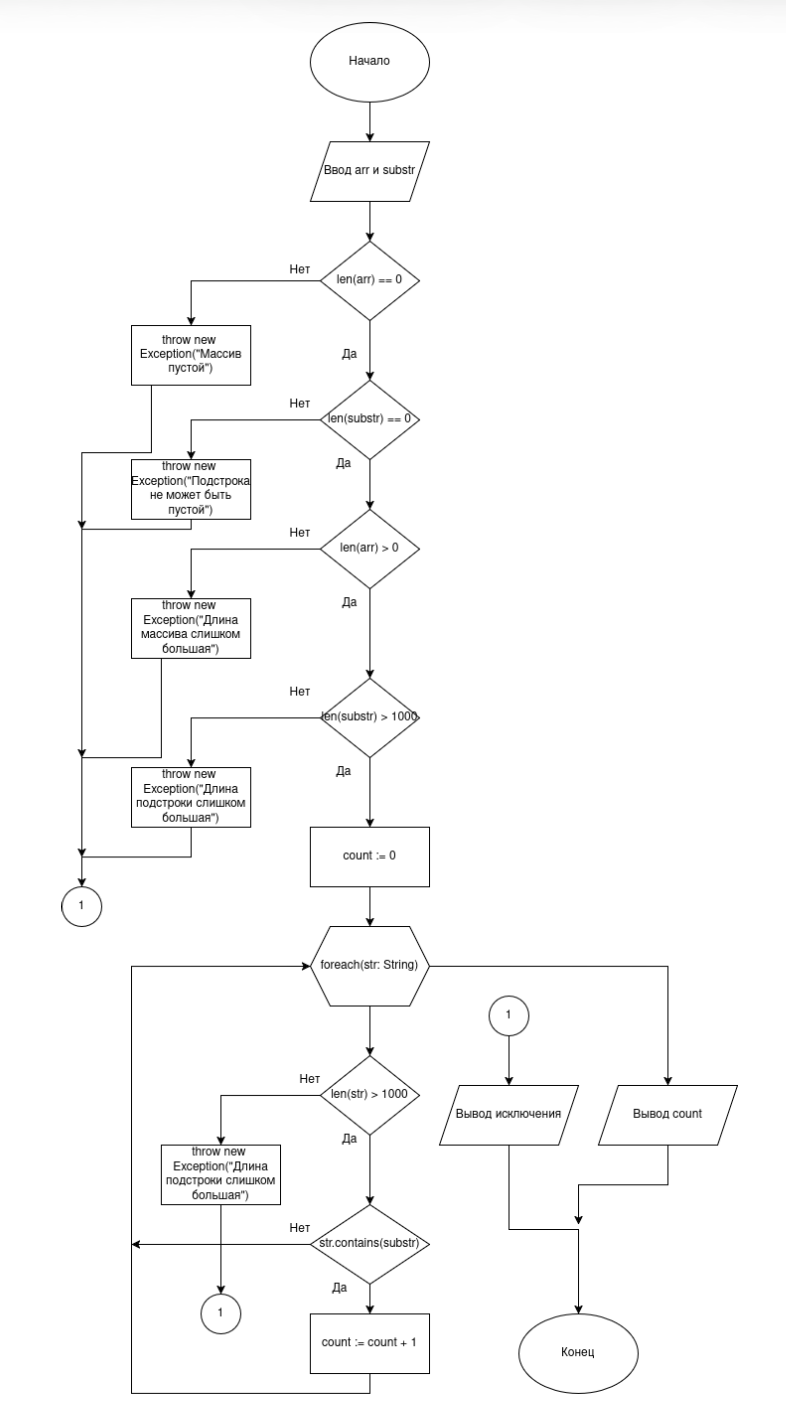
\includegraphics[width=0.8\textwidth]{pics/scheme2.png}
	\captionof{figure}{Блок-схема}
\end{figure}

\subsection{Тестирование методом <<чёрного>> ящика}
%-------------------------------------------------------------

\subsubsection{Разбиение на классы эквивалентности}

Исходя из ограничений программы составлено разбиение на классы эквивалентности по двум входным параметрам: \texttt{arr} и \texttt{substr}.

{\centering\large{
\begin{longtable}{|p{3.5cm}|p{5.5cm}|p{5.5cm}|}
    \caption{Классы эквивалентности для программы}\\
    \hline
    Входное условие & Допустимые классы & Недопустимые классы \\ \hline
    Массив \texttt{arr} &
        Массив из 1 элемента (1) &
        Пустой массив (7) \\ \hline
    &
        Массив из 2--99 элементов (2) &
        Массив из более чем 100 элементов (8) \\ \hline
    &
        Массив ровно из 100 элементов (3) &
        Массив, содержащий строку длиной $> 1000$ (9) \\ \hline
    Подстрока \texttt{substr} &
        Непустая подстрока, встречающаяся в \texttt{arr} (4) &
        Пустая строка (10) \\ \hline
    &
        Непустая подстрока, не встречающаяся в \texttt{arr} (5) &
        Подстрока длиной $> 1000$ (11) \\ \hline
    &
        Подстрока длиной ровно 1000 (6) &
        \\ \hline
\end{longtable}}}

В таблице~\ref{tab:equiv-tests} представлены тесты, покрывающие все классы эквивалентности.

{\centering\large{
\begin{longtable}{|c|p{3.5cm}|p{2.5cm}|p{3cm}|p{3cm}|p{1.5cm}|}
    \caption{Тесты по классам эквивалентности}
    \label{tab:equiv-tests}\\
    \hline
    N & \texttt{arr} & \texttt{substr} & Ожидаемый результат & Фактический результат & Результат \\ \hline
    1 &
        \texttt{\{"hello"\}} &
        \texttt{"he"} &
        \texttt{count = 1} &
        \texttt{count = 1} &
        Пройден \\ \hline
    2 &
        \texttt{\{"hello",} \texttt{"world",} \texttt{"hi"\}} &
        \texttt{"h"} &
        \texttt{count = 2} &
        \texttt{count = 2} &
        Пройден \\ \hline
    3 &
        Массив из 100 элементов \texttt{"a"} &
        \texttt{"a"} &
        \texttt{count = 100} &
        \texttt{count = 100} &
        Пройден \\ \hline
    4 &
        \texttt{\{"hello",} \texttt{"world"\}} &
        \texttt{"world"} &
        \texttt{count = 1} &
        \texttt{count = 1} &
        Пройден \\ \hline
    5 &
        \texttt{\{"hello",} \texttt{"world"\}} &
        \texttt{"xyz"} &
        \texttt{count = 0} &
        \texttt{count = 0} &
        Пройден \\ \hline
    6 &
        \texttt{\{"hello"\}} &
        \texttt{substr} дл. 1000 &
        \texttt{count = 0} &
        \texttt{count = 0} &
        Пройден \\ \hline
    7 &
        \texttt{\{\}} &
        \texttt{"he"} &
        Ошибка: массив пустой &
        Ошибка: массив пустой &
        Пройден \\ \hline
    8 &
        Массив из 101 эл. &
        \texttt{"a"} &
        Ошибка: массив слишком большой &
        Ошибка: массив слишком большой &
        Пройден \\ \hline
    9 &
        \texttt{\{строка} дл. 1001\texttt{\}} &
        \texttt{"he"} &
        Ошибка: строка слишком длинная &
        Ошибка: строка слишком длинная &
        Пройден \\ \hline
    10 &
        \texttt{\{"hello"\}} &
        \texttt{""} &
        Ошибка: пустая подстрока &
        Ошибка: пустая подстрока &
        Пройден \\ \hline
    11 &
        \texttt{\{"hello"\}} &
        \texttt{substr} дл. 1001 &
        Ошибка: подстрока слишком длинная &
        Ошибка: подстрока слишком длинная &
        Пройден \\ \hline
\end{longtable}}}

Все 11 тестов прошли успешно.

\subsubsection{Анализ граничных условий}

Исходя из ограничений программы выделяются следующие граничные значения:

\begin{enumerate}
    \item Размер массива: $0$ (пустой), $1$ (минимальный допустимый), $100$ (максимальный допустимый), $101$ (первый недопустимый).
    \item Длина строки в массиве: $1$ (минимальная), $1000$ (максимальная), $1001$ (первая недопустимая).
    \item Длина подстроки: $0$ (пустая --- недопустима), $1$ (минимальная допустимая), $1000$ (максимальная), $1001$ (первая недопустимая).
    \item Количество совпадений: $0$ (нет вхождений), $1$, все элементы.
\end{enumerate}

Для каждой из границ составлены тесты, соответствующие граничным значениям.

\begin{table}[H]
\centering
\caption{Проверка граничных условий}
\begin{tabular}{|c|p{3.5cm}|p{2.5cm}|p{3cm}|p{3cm}|p{1.5cm}|}
\hline
\textbf{N} & \textbf{\texttt{arr}} & \textbf{\texttt{substr}} & \textbf{Ожидаемый результат} & \textbf{Фактический результат} & \textbf{Результат} \\
\hline
1 &
    \texttt{\{\}} &
    \texttt{"a"} &
    Ошибка: массив пустой &
    Ошибка: массив пустой &
    Пройден \\
\hline
2 &
    \texttt{\{"a"\}} &
    \texttt{"a"} &
    \texttt{count = 1} &
    \texttt{count = 1} &
    Пройден \\
\hline
3 &
    Массив из 100 эл. \texttt{"a"} &
    \texttt{"a"} &
    \texttt{count = 100} &
    \texttt{count = 100} &
    Пройден \\
\hline
4 &
    Массив из 101 эл. &
    \texttt{"a"} &
    Ошибка: массив слишком большой &
    Ошибка: массив слишком большой &
    Пройден \\
\hline
5 &
    \texttt{\{"a"\}} (дл. строки $= 1$) &
    \texttt{"a"} &
    \texttt{count = 1} &
    \texttt{count = 1} &
    Пройден \\
\hline
6 &
    \texttt{\{"a"\}} \{str дл. 1000\} &
    \texttt{"a"} &
    \texttt{count = 1000} &
    \texttt{count = 1000} &
    Пройден \\
\hline
7 &
    \{str дл. 1001\} &
    \texttt{"a"} &
    Ошибка: строка слишком длинная &
    Ошибка: строка слишком длинная &
    Пройден \\
\hline
8 &
    \texttt{\{"hello"\}} &
    \texttt{""} &
    Ошибка: пустая подстрока &
    Ошибка: пустая подстрока &
    Пройден \\
\hline
9 &
    \texttt{\{"hello"\}} &
    \texttt{"h"} (дл. 1) &
    \texttt{count = 1} &
    \texttt{count = 1} &
    Пройден \\
\hline
10 &
    \texttt{\{"hello"\}} &
    \texttt{substr} дл. 1000 &
    \texttt{count = 0} &
    \texttt{count = 0} &
    Пройден \\
\hline
11 &
    \texttt{\{"hello"\}} &
    \texttt{substr} дл. 1001 &
    Ошибка: подстрока слишком длинная &
    Ошибка: подстрока слишком длинная &
    Пройден \\
\hline
12 &
    \texttt{\{"a" "b" "c"\}} &
    \texttt{"x"} &
    \texttt{count = 0} &
    \texttt{count = 0} &
    Пройден \\
\hline
13 &
    \texttt{\{"a" "a" "a"\}} &
    \texttt{"a"} &
    \texttt{count = 3} (все) &
    \texttt{count = 3} &
    Пройден \\
\hline
\end{tabular}
\end{table}

Все 13 тестов прошли успешно.

\subsubsection{Причинно-следственная диаграмма}

Для построения причинно-следственной диаграммы введём следующие обозначения.

\textbf{Причины:}
\begin{enumerate}
    \item Массив \texttt{arr} не пуст (размер $\ge 1$).
    \item Размер массива \texttt{arr} $\le 100$.
    \item Подстрока \texttt{substr} не пуста (длина $\ge 1$).
    \item Длина подстроки \texttt{substr} $\le 1000$.
    \item Все строки в массиве \texttt{arr} имеют длину от $1$ до $1000$ включительно.
\end{enumerate}

\textbf{Следствия:}
\begin{enumerate}
    \setcounter{enumi}{20}
    \item Программа генерирует исключение с сообщением \texttt{"Массив пустой"}.
    \item Программа генерирует исключение с сообщением \texttt{"Массив слишком большой"}.
    \item Программа генерирует исключение с сообщением \texttt{"Подстрока не может быть пустой"}.
    \item Программа генерирует исключение с сообщением \texttt{"Подстрока слишком длинная"}.
    \item Программа генерирует исключение с сообщением \texttt{"Слишком длинная строка в массиве"}.
    \item Программа возвращает целое неотрицательное число \texttt{count} (количество вхождений).
\end{enumerate}

\textbf{Промежуточные узлы:}
\begin{enumerate}
    \setcounter{enumi}{10}
    \item Узел 11: Данные валидны для вычисления (все причины 1--5 истинны).
\end{enumerate}

\textbf{Логические связи:}
\begin{enumerate}
    \item Следствие 21 (пустой массив) истинно, если причина 1 ложна.
    \item Следствие 22 (массив слишком большой) истинно, если причина 1 истинна И причина 2 ложна.
    \item Следствие 23 (пустая подстрока) истинно, если причины 1 и 2 истинны И причина 3 ложна.
    \item Следствие 24 (подстрока слишком длинная) истинно, если причины 1--3 истинны И причина 4 ложна.
    \item Следствие 25 (недопустимая длина строки в массиве) истинно, если причины 1--4 истинны И причина 5 ложна.
    \item Следствие 26 (успешное вычисление) истинно, если все причины 1--5 истинны (узел 11 истинен).
\end{enumerate}

\begin{figure}[H]
	\centering
	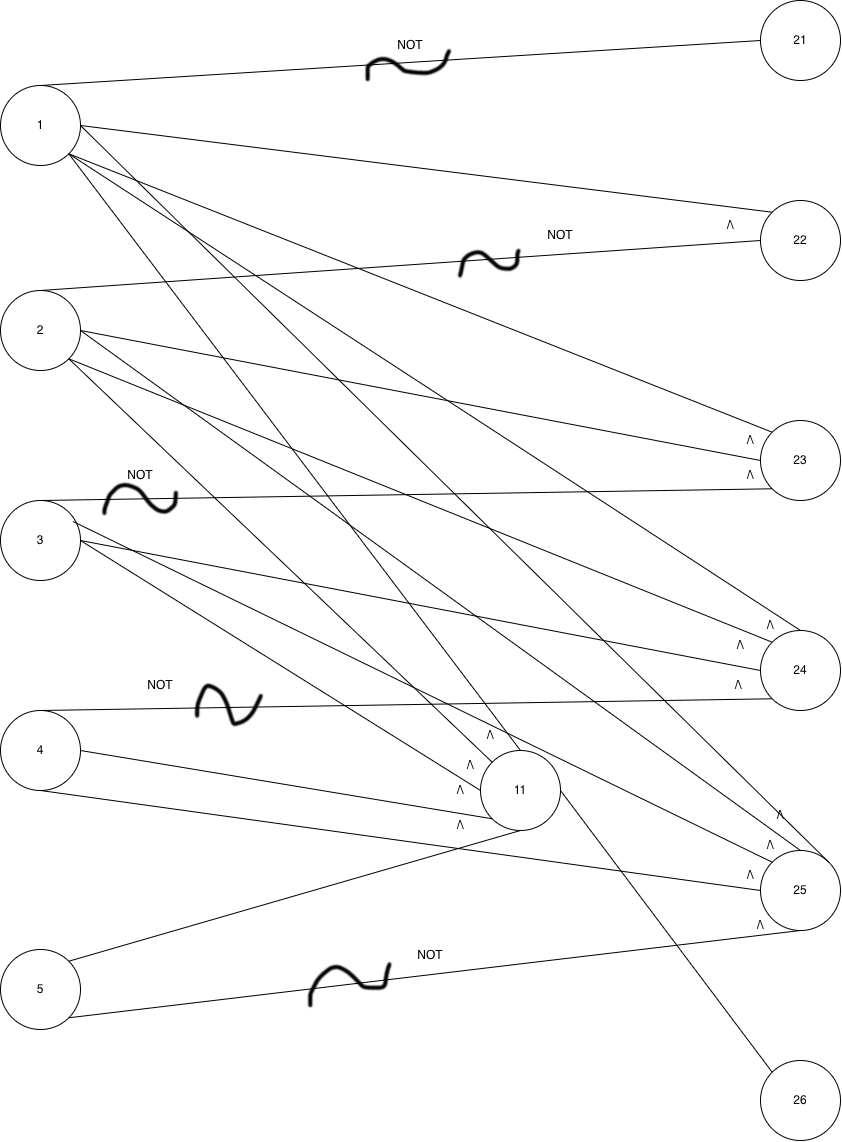
\includegraphics[width=0.8\textwidth]{../diagram1.png}
	\caption{Причинно-следственная диаграмма}
\end{figure}

\begin{table}[H]
\centering
\caption{Таблица решений}
\renewcommand{\arraystretch}{1.4}
\begin{tabular}{|l|c|c|c|c|c|c|c|}
\hline
 & \textbf{1} & \textbf{2} & \textbf{3} & \textbf{4} & \textbf{5} & \textbf{6} & \textbf{7} \\
\hline
Причина 1 (массив не пуст)          & 0 & 1 & 1 & 1 & 1 & 1 & 1 \\
\hline
Причина 2 (размер $\le 100$)        & -- & 0 & 1 & 1 & 1 & 1 & 1 \\
\hline
Причина 3 (подстрока не пуста)      & -- & -- & 0 & 1 & 1 & 1 & 1 \\
\hline
Причина 4 (длина подстроки $\le 1000$) & -- & -- & -- & 0 & 1 & 1 & 1 \\
\hline
Причина 5 (длины строк в $[1,1000]$)   & -- & -- & -- & -- & 0 & 1 & 1 \\
\hline
Узел 11 (все причины истинны)       & 0 & 0 & 0 & 0 & 0 & 1 & 1 \\
\hline
Следствие 21 (пустой массив)        & 1 & 0 & 0 & 0 & 0 & 0 & 0 \\
\hline
Следствие 22 (массив слишком большой) & 0 & 1 & 0 & 0 & 0 & 0 & 0 \\
\hline
Следствие 23 (пустая подстрока)     & 0 & 0 & 1 & 0 & 0 & 0 & 0 \\
\hline
Следствие 24 (подстрока слишком длинная) & 0 & 0 & 0 & 1 & 0 & 0 & 0 \\
\hline
Следствие 25 (недопустимая строка)  & 0 & 0 & 0 & 0 & 1 & 0 & 0 \\
\hline
Следствие 26 (успех, count)         & 0 & 0 & 0 & 0 & 0 & 1 & 1 \\
\hline
\end{tabular}
\end{table}

\begin{table}[H]
\centering
\caption{Тесты на основе таблицы решений}
\renewcommand{\arraystretch}{1.5}
\begin{tabular}{|c|p{3cm}|p{3cm}|p{3cm}|p{3cm}|c|}
\hline
\textbf{N} & \textbf{Комбинация} & \textbf{Входные данные} & \textbf{Ожидаемый рез.} & \textbf{Фактич. рез.} & \textbf{Результат} \\
\hline
1 & $0$ & \texttt{arr = \{\}, substr = "he"} & Исключение: \texttt{"Массив пустой"} & Исключение: \texttt{"Массив пустой"} & Пройден \\
\hline
2 & $1,\ 0$ & \texttt{arr размера 101, substr = "e"} & Исключение: \texttt{"Массив слишком большой"} & Исключение: \texttt{"Массив слишком большой"} & Пройден \\
\hline
3 & $1,\ 1,\ 0$ & \texttt{arr = \{"hello"\}, substr = ""} & Исключение: \texttt{"Подстрока не может быть пустой"} & Исключение: \texttt{"Подстрока не может быть пустой"} & Пройден \\
\hline
4 & $1,\ 1,\ 1,\ 0$ & \texttt{arr = \{"test"\}, substr длины 1001} & Исключение: \texttt{"Подстрока слишком длинная"} & Исключение: \texttt{"Подстрока слишком длинная"} & Пройден \\
\hline
5 & $1,\ 1,\ 1,\ 1,\ 0$ & \texttt{arr = \{"a"*1001\}, substr = "e"} & Исключение: \texttt{"Слишком длинная строка в массиве"} & Исключение: \texttt{"Слишком длинная строка в массиве"} & Пройден \\
\hline
6 & $1,\ 1,\ 1,\ 1,\ 1$ & \texttt{arr = \{"hello", "world"\}, substr = "o"} & Возврат \texttt{count = 2} & Возврат \texttt{count = 2} & Пройден \\
\hline
\end{tabular}
\end{table}


\subsubsection{Результаты тестирования программы №2 методом чёрного ящика}

В результате тестирования методом чёрного ящика было составлено 31 тест.
Все тесты прошли успешно.

Тестирование по классам эквивалентности охватило все выделенные допустимые и недопустимые классы
для входных параметров \texttt{arr} и \texttt{substr}. Анализ граничных условий выявил корректность
обработки крайних значений по всем трём измерениям: размеру массива, длине строки и длине подстроки.
Тестирование на основе таблицы решений верифицировало каждое следствие в отдельности.


\subsection{Тестирование методом белого ящика}

Алгоритм составления тестов методом «белого» ящика предполагает обход всех
возможных путей в теле программы и проверку выполнения каждого оператора не
менее одного раза.

В программе можно выделить следующие ключевые условия и соответствующие
им ветви:

\begin{enumerate}
    \item Условие C1: (\texttt{len(arr) == 0}):

        Ветвь T (True): Выход из программы с ошибкой «Массив пустой».

        Ветвь F (False): Продолжение выполнения.

    \item Условие C2: (\texttt{len(substr) == 0}):

        Ветвь T (True): Выход из программы с ошибкой «Подстрока не может быть пустой».

        Ветвь F (False): Продолжение выполнения.

    \item Условие C3: (\texttt{len(arr) > 100}) (проверка размера массива):

        Ветвь T (True): Выход из программы с ошибкой «Длина массива слишком большая».

        Ветвь F (False): Продолжение выполнения.

    \item Условие C4: (\texttt{len(substr) > 1000}) (проверка длины подстроки):

        Ветвь T (True): Выход из программы с ошибкой «Длина подстроки слишком большая».

        Ветвь F (False): Продолжение выполнения.

    \item Условие C5: (\texttt{len(str) > 1000}) (внутри цикла \texttt{foreach}):

        Ветвь T (True): Выход из программы с ошибкой «Длина строки слишком большая».

        Ветвь F (False): Продолжение проверки или выход из цикла.

    \item Условие C6: (\texttt{str.contains(substr)}):

        Ветвь T (True): Увеличение счётчика \texttt{count}.

        Ветвь F (False): Переход к следующему элементу.
\end{enumerate}

\noindent \textbf{Возможные пути выполнения:}

\begin{enumerate}
    \item Пустой массив: C1(T) $\to$ Завершение.
    \item Пустая подстрока: C1(F) $\to$ C2(T) $\to$ Завершение.
    \item Массив слишком большой: C1(F) $\to$ C2(F) $\to$ C3(T) $\to$ Завершение.
    \item Подстрока слишком длинная: C1(F) $\to$ C2(F) $\to$ C3(F) $\to$ C4(T) $\to$ Завершение.
    \item Строка в массиве слишком длинная: C1(F) $\to$ \ldots $\to$ C4(F) $\to$ цикл $\to$ C5(T) $\to$ Завершение.
    \item Успешный поиск (есть совпадения): C1(F) $\to$ \ldots $\to$ C4(F) $\to$ цикл $\to$ C5(F) $\to$ C6(T) $\to$ \ldots $\to$ выход из цикла $\to$ Вывод \texttt{count}.
    \item Поиск без совпадений: C1(F) $\to$ \ldots $\to$ C4(F) $\to$ цикл $\to$ C5(F) $\to$ C6(F) $\to$ \ldots $\to$ выход из цикла $\to$ Вывод \texttt{count = 0}.
    \item Смешанный поиск: C1(F) $\to$ \ldots $\to$ C4(F) $\to$ цикл с многократным выполнением C5(F), C6(T/F) $\to$ выход из цикла $\to$ Вывод \texttt{count}.
\end{enumerate}

\subsubsection{Покрытие операторов}

Критерием покрытия является выполнение каждого оператора программы хотя
бы один раз. Это необходимое, но не достаточное условие для приемлемого тестирования по принципу белого ящика.

Для покрытия всех операторов достаточно одного теста, который пройдёт по
основному пути и не вызовет досрочных завершений. Для этого каждой возможной ветви присвоим обозначения A-L и выберем маршрут,
проходящий по пути ACEGIK.

\begin{table}[h!]
\centering
\caption{Покрытие операторов}
\begin{tabularx}{\textwidth}{|c|c|X|X|X|X|X|c|c|}
\hline
\textbf{N} & \textbf{arr} & \textbf{substr} & Путь & \textbf{Ожид. результат} & \textbf{Факт. результат} & \textbf{Путь} & \textbf{Статус} \\
\hline
1 & \{"hello","world","hello"\} & "he" & ACEGIK & 2 & 2 & 6 & Пройден \\
\hline
\end{tabularx}
\end{table}

Тест №1 выполнил все операторы программы.

\subsubsection{Покрытие решений}

В соответствии с этим критерием необходимо составить такой набор тестов, при
котором каждое условие в программе примет как истинное, так и ложное значения.
Таким образом, к тестам, составленным для метода покрытия операторов, необходимо добавить тесты, которые будут проверять все возможные переходы.

Тесты, покрывающие все решения программы, представлены ниже.

\begin{table}[h!]
\centering
\caption{Покрытие решений}
\begin{tabularx}{\textwidth}{|c|X|X|X|X|c|c|c|c|c|c|c|}
\hline
\textbf{N} & \textbf{arr} & \textbf{substr} & \textbf{Ожид. рез.} & \textbf{Факт. рез.} & \textbf{C1} & \textbf{C2} & \textbf{C3} & \textbf{C4} & \textbf{C5} & \textbf{C6} & \textbf{Статус} \\
\hline
1 & \{"hello","world","hello"\} & "he" & 2 & 2 & F & F & F & F & F & T & Пройден \\
\hline
2 & \{"cat","dog"\} & "xyz" & 0 & 0 & F & F & F & F & F & F & Пройден \\
\hline
3 & \{\} & "he" & Ошибка: массив пустой & Ошибка: массив пустой & T & -- & -- & -- & -- & -- & Пройден \\
\hline
4 & \{"hello"\} & "" & Ошибка: пустая подстрока & Ошибка: пустая подстрока & F & T & -- & -- & -- & -- & Пройден \\
\hline
5 & arr из 101 эл. & "a" & Ошибка: массив слишком большой & Ошибка: массив слишком большой & F & F & T & -- & -- & -- & Пройден \\
\hline
6 & \{"hello"\} & substr дл. 1001 & Ошибка: подстрока слишком длинная & Ошибка: подстрока слишком длинная & F & F & F & T & -- & -- & Пройден \\
\hline
7 & \{"hello", str дл. 1001\} & "he" & Ошибка: строка слишком длинная & Ошибка: строка слишком длинная & F & F & F & F & T & -- & Пройден \\
\hline
\end{tabularx}
\end{table}

Тест №1: Проверяет C1=F, C2=F, C3=F, C4=F, C5=F, C6=T.

Тест №2: Проверяет C6=F, а также выход из цикла без совпадений.

Тест №3: Проверяет C1=T.

Тест №4: Проверяет C2=T.

Тест №5: Проверяет C3=T.

Тест №6: Проверяет C4=T.

Тест №7: Проверяет C5=T.

Все условия были протестированы на T и F.

\subsubsection{Покрытие условий}

В соответствии с этим критерием количество тестов должно быть таким, чтобы
все возможные результаты каждого условия в решении выполнялись по крайней мере
один раз.

\begin{table}[h!]
\centering
\caption{Покрытие условий}
\begin{tabularx}{\textwidth}{|c|X|X|X|X|c|c|c|}
\hline
\textbf{N} & \textbf{arr} & \textbf{substr} & \textbf{Ожид. рез.} & \textbf{Факт. рез.} & \textbf{C1} & \textbf{C2} & \textbf{Статус} \\
\hline
1 & \{"hello","world"\} & "he" & 1 & 1 & F & F & Пройден \\
\hline
2 & \{\} & "he" & Ошибка: массив пустой & Ошибка: массив пустой & T & -- & Пройден \\
\hline
3 & \{"hello"\} & "" & Ошибка: пустая подстрока & Ошибка: пустая подстрока & F & T & Пройден \\
\hline
\end{tabularx}
\end{table}

Тест №1: C1=F, C2=F.

Тест №2: C1=T.

Тест №3: C2=T.

Все элементарные условия были проверены на T и F.

\subsubsection{Покрытие решений и условий}

Согласно этому критерию набор тестов является достаточно полным, если удовлетворяются следующие требования: каждое условие в решении принимает каждое
возможное значение по крайней мере один раз, каждый возможный исход решения
проверяется по крайней мере один раз и каждой точке входа управление передаётся
по крайней мере один раз.

Тесты, написанные ранее, обеспечивают покрытие решений и условий.

\begin{table}[h!]
\centering
\caption{Покрытие решений и условий}
\begin{tabularx}{\textwidth}{|c|X|X|X|X|c|c|c|c|c|c|c|}
\hline
\textbf{N} & \textbf{arr} & \textbf{substr} & \textbf{Ож. рез.} & \textbf{Факт. рез.} & \textbf{C1} & \textbf{C2} & \textbf{C3} & \textbf{C4} & \textbf{C5} & \textbf{C6} & \textbf{Статус} \\
\hline
1 & \{"hello","world","hello"\} & "he" & 2 & 2 & F & F & F & F & F & T & Пройден \\
\hline
2 & \{"cat","dog"\} & "xyz" & 0 & 0 & F & F & F & F & F & F & Пройден \\
\hline
3 & \{\} & "he" & Ошибка: массив пустой & Ошибка: массив пустой & T & -- & -- & -- & -- & -- & Пройден \\
\hline
4 & \{"hello"\} & "" & Ошибка: пустая подстрока & Ошибка: пустая подстрока & F & T & -- & -- & -- & -- & Пройден \\
\hline
5 & arr из 101 эл. & "a" & Ошибка: массив слишком большой & Ошибка: массив слишком большой & F & F & T & -- & -- & -- & Пройден \\
\hline
6 & \{"hello"\} & substr дл. 1001 & Ошибка: подстрока слишком длинная & Ошибка: подстрока слишком длинная & F & F & F & T & -- & -- & Пройден \\
\hline
7 & \{"hello", str дл. 1001\} & "he" & Ошибка: строка слишком длинная & Ошибка: строка слишком длинная & F & F & F & F & T & -- & Пройден \\
\hline
\end{tabularx}
\end{table}

Все решения и условия покрыты.

\subsubsection{Комбинаторное покрытие условий}

Этот критерий требует создания такого набора тестов, при котором каждая возможная комбинация результатов вычисления условий в каждом решении и каждая
точка входа проверяются по крайней мере один раз.

Для условия C1 (\texttt{len(arr) == 0}) и C2 (\texttt{len(substr) == 0}) возможны следующие комбинации: (F,F), (T,--), (F,T). Условие C2 не вычисляется при C1=T, поэтому комбинация (T,T) недостижима.

\begin{table}[H]
\centering
\caption{Комбинаторное покрытие условий}
\begin{tabularx}{\textwidth}{|c|X|X|X|X|c|c|c|}
\hline
\textbf{N} & \textbf{arr} & \textbf{substr} & \textbf{Ожид. рез.} & \textbf{Факт. рез.} & \textbf{C1} & \textbf{C2} & \textbf{Статус} \\
\hline
1 & \{"hello","world","hello"\} & "he" & 2 & 2 & F & F & Пройден \\
\hline
2 & \{\} & "he" & Ошибка: массив пустой & Ошибка: массив пустой & T & -- & Пройден \\
\hline
3 & \{"hello"\} & "" & Ошибка: пустая подстрока & Ошибка: пустая подстрока & F & T & Пройден \\
\hline
4 & arr из 101 эл. & "a" & Ошибка: массив слишком большой & Ошибка: массив слишком большой & F & F (C3=T) & Пройден \\
\hline
5 & \{"hello"\} & substr дл. 1001 & Ошибка: подстрока слишком длинная & Ошибка: подстрока слишком длинная & F & F (C4=T) & Пройден \\
\hline
6 & \{"hello", str дл. 1001\} & "he" & Ошибка: строка слишком длинная & Ошибка: строка слишком длинная & F & F (C5=T) & Пройден \\
\hline
7 & \{"cat","dog"\} & "xyz" & 0 & 0 & F & F (C6=F) & Пройден \\
\hline
\end{tabularx}
\end{table}

Все достижимые комбинации условий покрыты. Комбинация C1=T и C2=T недостижима, так как при истинности C1 программа завершается до проверки C2.

\subsubsection{Результаты тестирования методом белого ящика}

В ходе тестирования алгоритма подсчёта вхождений подстроки в массиве строк были разработаны тесты для различных критериев покрытия кода.

Для покрытия операторов был составлен один тест с входными данными \texttt{arr = \{"hello", "world", "hello"\}} и \texttt{substr = "he"}. Ожидаемый результат \texttt{count = 2} совпал с фактическим, тест пройден. Этот тест выполнил все операторы программы, включая инициализацию счётчика, цикл \texttt{foreach} и проверку вхождения подстроки, однако не проверил ветви исключений.

Для покрытия решений потребовалось семь тестов. Первый тест с \texttt{arr = \{"hello","world","hello"\}} и \texttt{substr = "he"} дал результат \texttt{count = 2}, проверены условия C1=ложь, C2=ложь, C3=ложь, C4=ложь, C5=ложь, C6=истина. Второй тест с \texttt{arr = \{"cat","dog"\}} и \texttt{substr = "xyz"} дал результат \texttt{count = 0}, проверено условие C6=ложь и выход из цикла без совпадений. Третий тест с пустым массивом \texttt{arr = \{\}} проверил C1=истина и выдал сообщение об ошибке «Массив пустой». Четвёртый тест с \texttt{substr = ""} проверил C2=истина и выдал ошибку «Подстрока не может быть пустой». Пятый тест с массивом из 101 элемента проверил C3=истина и выдал ошибку «Длина массива слишком большая». Шестой тест с подстрокой длиной 1001 символ проверил C4=истина и выдал ошибку «Длина подстроки слишком большая». Седьмой тест с массивом, содержащим строку длиной 1001 символ, проверил C5=истина и выдал ошибку «Длина строки слишком большая». Все тесты пройдены.

Для покрытия условий протестированы элементарные условия C1 и C2. Тест с корректными входными данными проверил комбинацию C1=ложь, C2=ложь. Тест с пустым массивом проверил C1=истина. Тест с пустой подстрокой проверил C2=истина. Все тесты пройдены, программа выдала ожидаемые результаты.

Для покрытия решений и условий использованы все вышеперечисленные тесты. Каждое условие C1–C6 было проверено как на истинное, так и на ложное значение, а каждый возможный исход каждого решения покрыт хотя бы одним тестом. Все семь тестов пройдены.

Для комбинаторного покрытия условий проверены все достижимые комбинации для условий C1 и C2: (ложь, ложь) с корректными входными данными, (истина, --) с пустым массивом, (ложь, истина) с пустой подстрокой. Комбинация (истина, истина) недостижима, так как при C1=истина программа завершается до вычисления C2. Дополнительно покрыты все ветви условий C3–C6. Все тесты пройдены.

\pagebreak

\section{Заключение}

В ходе выполнения данной лабораторной работы были изучены и применены методы тестирования
«белым ящиком» и «чёрным ящиком» для обеих программ.

\textbf{Программа №1 (проверка простоты числа).}
Тестирование методом «чёрного ящика» включало 29 тестов: 12 по классам эквивалентности,
11 по граничным значениям и 6 по таблице решений. Все тесты пройдены успешно.
Тестирование методом «белого ящика» включало 6 тестов, охватывающих пять критериев покрытия. 
Все 7 достижимых комбинаций условий C1--C6 покрыты. Дефектов обнаружено не было.

\textbf{Программа №2 (подсчёт вхождений подстроки).}
Тестирование методом «чёрного ящика» включало 31 тест: 11 по классам эквивалентности,
13 по граничным значениям и 7 по таблице решений. Все тесты пройдены успешно.
Тестирование методом «белого ящика» включало 7 тестов, охватывающих пять критериев покрытия
кода. Комбинация C1=T, C2=T признана недостижимой вследствие раннего завершения программы
при C1=T. Все тесты пройдены успешно.

По итогам выполненной работы можно сделать вывод, что оба метода тестирования дополняют
друг друга и в совокупности обеспечивают высокое качество проверки программного обеспечения.
Метод «белого ящика» позволяет убедиться в корректности внутренней логики и полноте охвата
всех ветвей кода. Метод «чёрного ящика» проверяет соответствие поведения программы требованиям
спецификации без учёта внутренней реализации. Совместное применение обоих методов снижает
вероятность пропуска дефектов и обеспечивает комплексную верификацию программного продукта.

\pagebreak

\begin{thebibliography}{3}
	\bibitem{[1]} Майерс Г. <<Искусство тестирования программ>>, СПб, Диалектика, 2012г.
\end{thebibliography}


\end{document}